\begin{titlepage}
  \begin{center}
    \vspace{8cm}
    \Huge \textbf{Annexes}
  \end{center}
\end{titlepage}

\clearpage

\section*{Cahier des charges}\label{cdc}

\textit{Ce document rédigé par nos soins constitue le cahier des charges qui a été validé par nos clients début janvier 2013.}

\vspace{1cm}

Il a été souligné la nécessité de garder à l'esprit le public visé afin de le cibler au mieux - à savoir les professeurs de guitare d'une école de musique et leurs élèves, ainsi qu'une population de ``joueurs'' désirant s'initier ou s'améliorer à la guitare. L'interface et les fonctionnalités des logiciels du projet devront donc être adaptés en conséquence, en visant à la fois l'accessibilité et l'ergonomie. En outre, lors des entretiens avec les clients, de nombreux points ont été soulevés et soumis à notre évaluation. Nous les détaillerons dans cette partie.

\subsubsection*{Relatifs à l'ensemble du projet}

Les points suivants s'appliquent à l'ensemble du projet, c'est-à-dire à la fois à l'éditeur et au player.
\begin{itemize}
 \item \underline{Deux logiciels :} les parties éditeur et player devront être séparées en deux exécutables
 \begin{itemize}
  \item De cette façon, l'éditeur sera réservé au professeur.
  \item Le player sera quant à lui accessible au professeur et à son élève.
 \end{itemize}
 \item \underline{Mac OS X et Windows :} le projet devra pouvoir être utilisable intégralement sur ces deux systèmes d'exploitation.
 \begin{itemize}
  \item A cet effet, nous reprendrons les bibliothèques Qt, FMOD et Portaudio utilisées dans les précédentes versions du logiciel, et qui ont l'avantage d'être multi-OS.
  \item Le livrable sera fourni sous la forme d'un installateur pour chacun de ces OS.
 \end{itemize}
 \item \underline{Interface :} comme il a été souligné précédemment, un soin particulier sera attaché à l'interface utilisateur pour la rendre la plus intuitive et attrayante possible.
 \begin{itemize}
  \item Pour cela, nous créerons une version traduite en Français
  \item Des menus d'aide seront également présents pour accompagner les utilisateurs
 \end{itemize}
 \item \underline{Version finale :} le logiciel devra être fini et prêt au déploiement dans l'école de musique cliente pour avril 2013.
\end{itemize}

\subsubsection*{Relatifs à l'éditeur}

Les besoins propres à l'éditeur et nos propositions pour y répondre sont énumérés dans cette partie. L'éditeur permettra la saisie des accords d'un morceau par le professeur directement dans une grille.

L'éditeur est destiné à créer une grille d'accords sans assistance. Il se présente sous la forme d'une grille dont chaque case correspond à une mesure, et chaque ligne à une phrase.

\begin{itemize}
 \item \underline{Saisie :} la saisie des accords se fait soit case par case, soit en sélectionnant directement toutes les cases correspondant au même accord.
 \begin{itemize}
  \item Les accords se rentrent soit à la main, soit à l'aide d'un menu listant tous les accords reconnus par le logiciel.
  \item Afin de faciliter la saisie, les derniers accords utilisés seront mis en évidence.
  \item L'utilisateur pourra également indiquer la tonalité du morceau qu'il veut saisir pour que soient mis en évidence les accords les plus utilisés pour cette tonalité.
 \end{itemize}
 \item \underline{Écoute :} pour l'aider lors de la saisie, l'utilisateur pourra écouter directement via l'éditeur le fichier mp3 qu'il aura sélectionné.
 \begin{itemize}
  \item Les fonctionnalités les plus courantes d'un lecteur audio seront implémentées, telles que la pause, la reprise et le retour en arrière.
  \item Il est à noter que cette lecture audio ne servira qu'à l'utilisateur, pas au logiciel. Néanmoins, le chemin vers ce fichier sera retenu afin de pouvoir le réutiliser en changeant de mode d'édition, ou lors de la lecture par le Player de la partition créée.
 \end{itemize}
 \item \underline{Synchronisation audio :} pour que la partition créée soit utilisable par le Player, il faut qu'une information de tempo soit précisée par l'utilisateur.
 \begin{itemize}
  \item Pour cela, l'utilisateur sera invité à ouvrir le fichier mp3 correspondant à sa saisie (s'il ne l'a pas déjà fait pour s'aider lors de cette même saisie).
  \item Une fenêtre l'invitera à démarrer le fichier mp3 et à appuyer deux fois sur la touche espace de son clavier.
  \item Ces deux appuis délimiteront la durée d'une case de la grille.
  \item Si besoin est, il pourra recommencer cette étape à sa guise.
  \item Cette étape est facultative si l'utilisateur ne souhaite pas utiliser sa partition sur le player.
 \end{itemize}
\end{itemize}

\underline{Fonctionnalités générales de l'éditeur}

Afin que l'utilisateur puisse accéder à n'importe quel moment aux partitions qu'il aura créées, il se verra offrir la possibilité d'exporter sa grille d'accords dans un fichier.

\begin{itemize}
 \item \underline{Export :} deux formats de fichiers seront utilisables pour sauvegarder la partition sur le disque dur de l'utilisateur.
 \begin{itemize}
  \item Un premier format dit “grille” adoptera les conventions de l'école de musique cliente et servira pour impression.
  \item Un second format basé sur le langage xml permettra l'utilisation de la partition sur le player. L'étape de synchronisation audio devra être validée au préalable.
  \item Ces deux formats ne sont pas incompatibles, c'est-à-dire que la partition pourra être sauvegardée aussi bien dans un format que dans l'autre, et pourquoi pas dans les deux en même temps.
 \end{itemize}
 \item \underline{Import :} pour permettre d'éditer une partition dont la saisie a déjà été commencée, il sera possible de charger un fichier grille ou xml généré préalablement par l'éditeur. La grille d'accords sera remplie comme il se doit avec les données du fichier.
\end{itemize}

L'interface devra également permettre une plus grande flexibilité que l'actuelle au niveau des morceaux. Il devra par exemple être possible de modifier le nombre de cases par ligne en cours de saisie, ainsi que de générer des partitions aux mesures irrégulières. Dans ce cas, l'export au format grille serait autorisé, mais celui au format xml nécessitera au préalable que l'utilisateur indique tous les changements de mesures ainsi que les durées de chaque case dans ces portions.

\subsubsection*{Relatifs au player}

La partie jouable du projet est déjà fonctionnelle. Il faudra cependant veiller à y apporter quelques nouveautés.

\begin{itemize}
 \item \underline{Deux modes :} un mode orienté jeu et un mode orienté apprentissage
 \begin{itemize}
  \item Le mode jeu se basera sur un score calculé en deux étapes
  \begin{itemize}
   \item A-t-il joué le bon accord?
   \item L'a-t-il tenu assez longtemps?
  \end{itemize}
  \item Le mode apprentissage bouclera sur les différentes parties du morceau jusqu'à ce que le joueur les réussisse parfaitement.
 \end{itemize}
 \item \underline{Interface :} plus attrayante et plus ergonomique
 \begin{itemize}
  \item Proposer un mode plein écran
  \item Indiquer au joueur son avancée dans la partition au cours de la partie
  \item Mode horizontal ou vertical
 \end{itemize}
 \item \underline{Enchaînement :} possibilité de jouer plusieurs morceaux à la suite
 \item \underline{Entrées audio :} gestion des différentes entrées audio de l'ordinateur.
 \begin{itemize}
  \item Une extension intéressante serait de développer un mode multijoueur.
 \end{itemize}
\end{itemize}


\begin{figure}[!ht]
\begin{center}
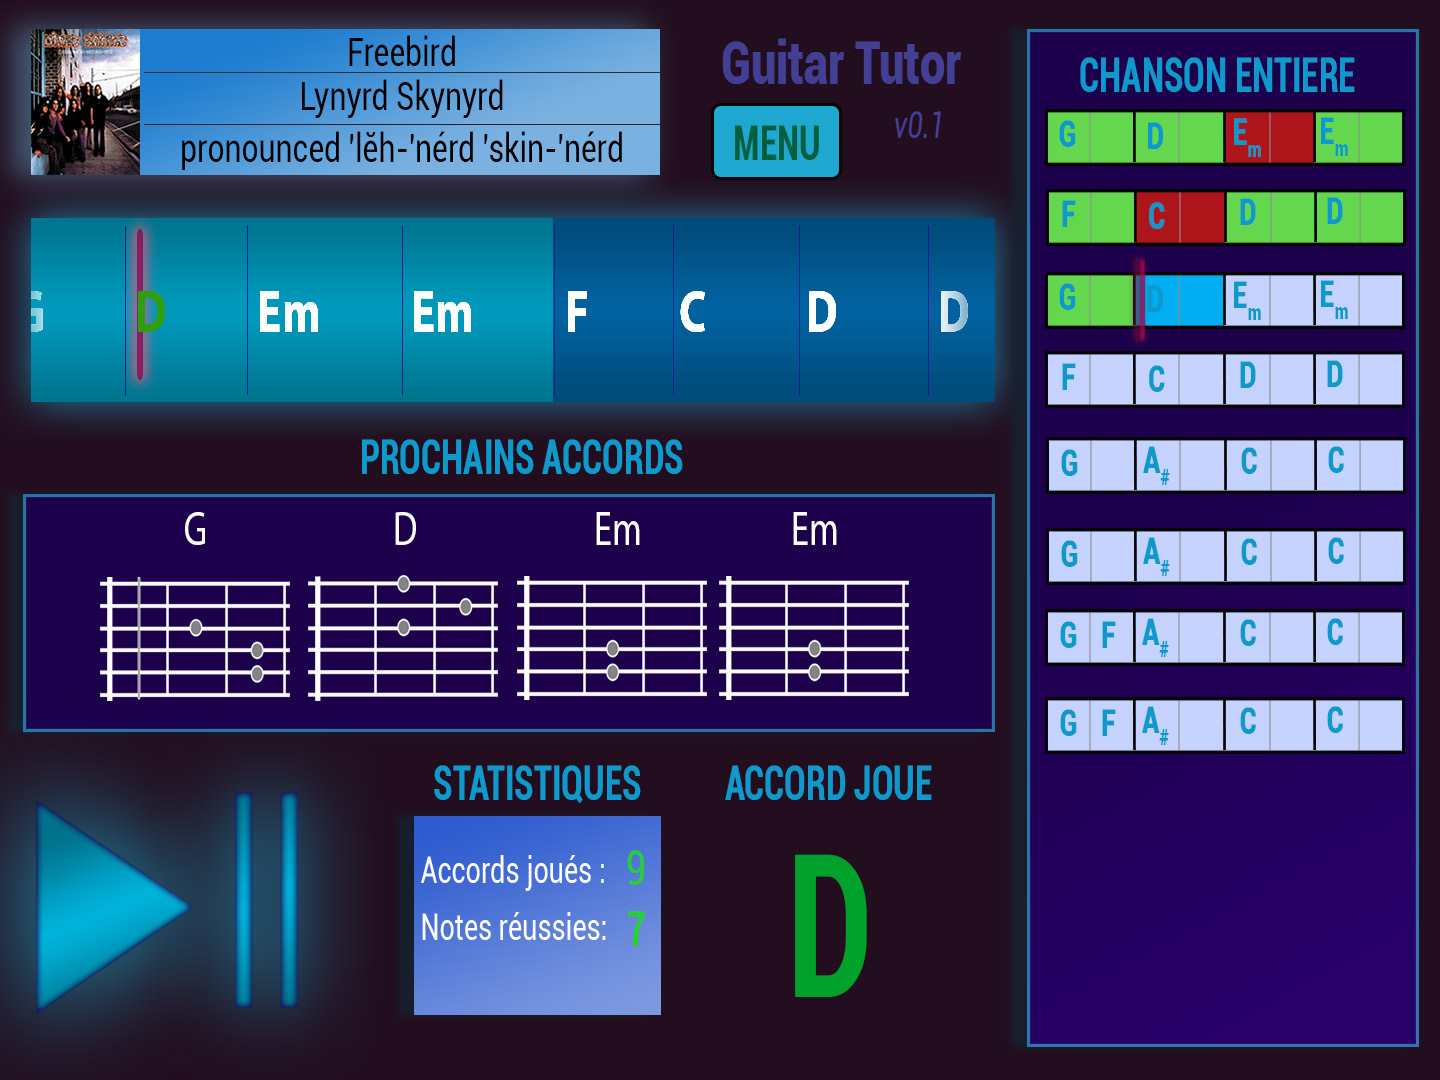
\includegraphics[width=450px]{interface_player_prototype.jpg}
\caption{Prototype d'interface pour le player}
\label{annexe_proto_player}
\end{center}
\end{figure}


\subsubsection*{API GuitarTutor}

Afin de faciliter la maintenance du code source et l'extension des fonctionnalités, nous axerons nos premières étapes de développement sur la création d'une API commune à l'éditeur et au player dans le but de respecter une architecture Modèle Vue Contrôleur (MVC). Cette méthode de développement n'ayant pas été utilisée par nos prédécesseurs, il nous faudra un certain temps pour reconstruire proprement le projet, mais nous sommes certains que cela sera un gain de temps pour la suite du développement.
